\begin{figure}[H]
  \centering
  \subfloat[$S = 50$ мкм; \textcolor{mygreen}{ по оси абсцисса - $\theta$ !}]{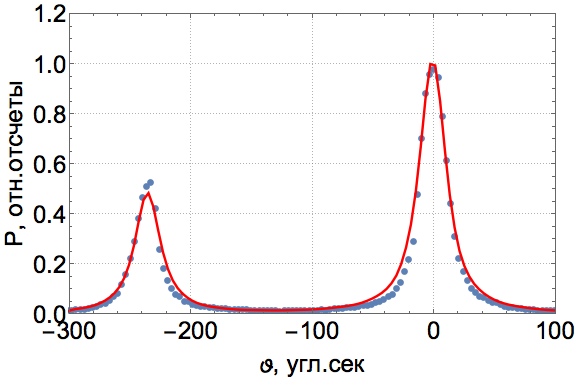
\includegraphics[width=0.7\textwidth]{images/single_cr_exp_s_005mm.png}}
  \hfill
  \subfloat[$S = 200$ мкм;]{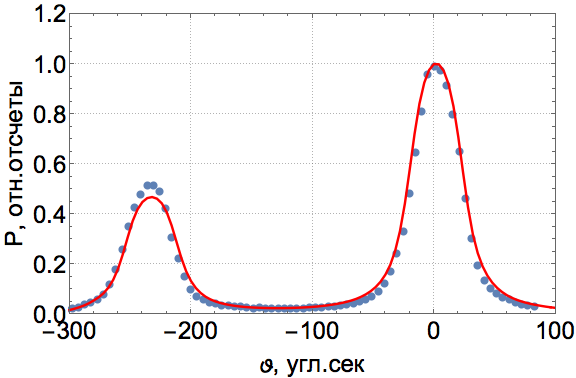
\includegraphics[width=0.7\textwidth]{images/single_cr_exp_s_02mm.png}}
  \caption{Однокристальный эксперимент, красный - расчет, синие точки - эксперимент}
  \label{ris:zero_exp}
\end{figure}
